\section{Phases, TODO}
\label{ProjMgmtMilestones}




\subsection{Project Phases and Milestones}
\label{sec:project_phases_milestones}

The following phases define blocks which can be closed after completing each of them.
The conclusion and start of each phase are used to review and adapt the current state.


\begin{itemize}

    \item \textbf{Phase 1, Research}
    \begin{itemize}
        \item Refine the problem statement.
        \item Define and narrow the scope.
        \item Define the use case.
        \item Conduct the literature review.
        \item Define the basic outlines for P2 to P3 and specify possible alternatives.
        \item Closure conditions:
        \begin{itemize}
            \item Research based on problem statement initially closed.
            \item Basis for P2 and P3 defined.
            \item Methodology for thesis defined.
            \item Review of baseline document parts from project 1 and 2 performed.
        \end{itemize}
    \end{itemize}

    \item \textbf{Phase 2, Define the Baseline with Stakeholders}
    \begin{itemize}
        \item Adapt P2 based on the findings from P1.
        \item Document the current stakeholder knowledge regarding error detection.
        \item Attempt to systematically identify and document relevant errors.
        \item Define how the results will be evaluated against future iterations.
        \item Closure Conditions
        \begin{itemize}
            \item Stakeholder knowledge documented
            \item Stakeholders have means to document errors.
            \item Defined test window during which manual and automatic errors are compared.
            \item Error documentation setup so that it is comparable to future Phase 3 implementation.
        \end{itemize}
    \end{itemize}


    \item \textbf{Phase 3, First Iteration}
    \begin{itemize}
        \item Review the results of P2 and adapt P3 accordingly.
        \item Define a minimal outline of the P3 objective while keeping the specific
              approach open to findings from the preceding research.
        \item Develop the data retrieval from AWS source.
        \item Develop the first/basic implementation.
        \item Summarise the results.
        \item Closure conditions
        \begin{itemize}
            \item The development environment is setup.
            \item Permissions required to work have been setup
            \item The MVP is setup and running.
            \item Data for test window retrieved.
            \item The Post stakeholders received presentation of current state.
            \item Defined test slot and registered test results
        \end{itemize}
    \end{itemize}

    \item \textbf{Phase 4, Second Iteration}
    \begin{itemize}
        \item Review the achievement of the objectives from P3 and, if necessary,
              pursue an alternative approach.
        \item Define a minimal outline of the phase objective while keeping the
              specific approach open to findings from the preceding research.
        \item Develop an adapted implementation.
        \item Summarise the results.
        \item Closure conditions
        \begin{itemize}
            \item Second iteration outline defined.
            \item Data for test window retrieved.
        \end{itemize}
    \end{itemize}

    \item \textbf{Phase 5, Comparative Evaluation}
    \begin{itemize}
        \item Compare the results of all investigated approaches.
        \item Identify factors that may limit a direct or fair comparison,
              including specific differences between the approaches.
    \end{itemize}

    \item \textbf{Phase 6, Analysis of Goal Achievement and Thesis Finalisation}
    \begin{itemize}
        \item Describe which objectives were achieved and which were not.
        \item Finalise the thesis document.
        \item Finalise the required deliverables:
        \begin{itemize}
            \item Video
            \item Poster
            \item Presentation and Defence
        \end{itemize}
        \item Milestone 11, Presentation ready
        \item Thesis document delivered
        \item Presentation held
    \end{itemize}

\end{itemize}



\begin{figure}[H]
    \centering
    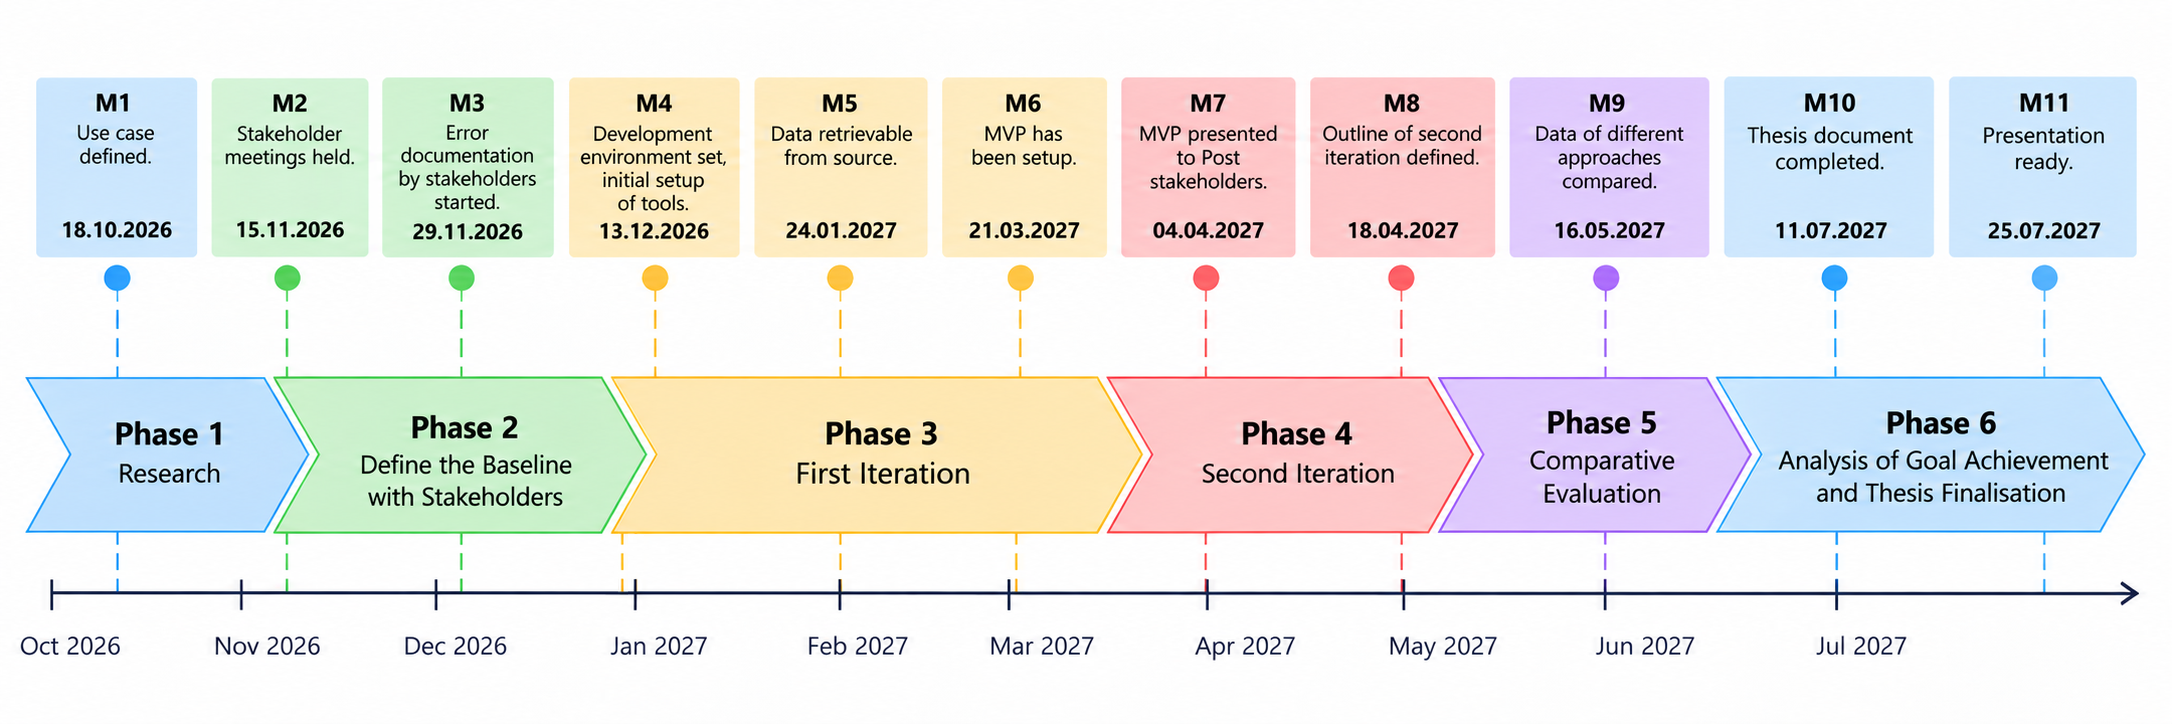
\includegraphics[width=0.8\textwidth]{./content/img/Mth/ProjectManagement/MilestoneTimelineAdapted_4.png}
    \caption{Milestones and phases defined at the start of the project}
    \label{fig:projmgmt_milestones_and_phases}
\end{figure}


\section{Milestones, TODO}
\label{ProjMgmtMilestones}



The milestones are events during the course of the phases. Each milestone will be
documented if it has been reached in time. Furthermore, any adaptations required to
the milestone plans have to be documented.

\subsection{Milestone Timeline}
\label{sec:milestone_timeline}

The milestone timelines are setup as follows before project start.

\begin{itemize}
    \item \textbf{Milestone 1:} Use case defined. -- \textbf{18.10.2026}
    \item \textbf{Milestone 2:} Stakeholder meetings held. -- \textbf{15.11.2026}
    \item \textbf{Milestone 3:} Error documentation by stakeholders started. -- \textbf{29.11.2026}
    \item \textbf{Milestone 4:} Development environment set, initial setup of tools -- \textbf{13.12.2026}
    \item \textbf{Milestone 5:} Data retrievable from source -- \textbf{24.01.2027}
    \item \textbf{Milestone 6:} MVP has been set up. -- \textbf{21.03.2027}
    \item \textbf{Milestone 7:} MVP presented to Post stakeholders. -- \textbf{04.04.2027}
    \item \textbf{Milestone 8:} Outline of second iteration defined. -- \textbf{18.04.2027}
    \item \textbf{Milestone 9:} Data of different approaches compared. -- \textbf{16.05.2027}
    \item \textbf{Milestone 10:} Thesis document completed. -- \textbf{11.07.2027}
    \item \textbf{Milestone 11:} Presentation ready -- \textbf{25.07.2027}
\end{itemize}

Todo,
Work for Future Roland
He will have to describe the milestones




\subsubsection*{Milestones}
The academic team manages the planning of the overall project timeline using milestones. These milestones define timeframes during which a section or chapter may be worked on. For this project, the following milestones have been defined:

\begin{itemize}
    \item Milestone 1: Basics completed
    \item Milestone 2: Completion of main research
    \item Milestone 3: Code implementation completed
    \item Milestone 4: Bug fixing completed
    \item Milestone 5: Submission of the project document
    \item Milestone 6: Presentation prepared
\end{itemize}

First, the basics ready refers to all the tools required to work being available. This step includes setting up LateX, setting milestones, setup of basic tool structure and definition of way of work. Second the main research done refers to the end of the purely theoretical part and start towards the solution design and the subsequent implementation of it. This comprises the main literature research being done. Third, the code done refers to the implementation of the solution being done. After this point no new features are to be implemented. Fourth, bug fix done comprises all corrections that had to be performed so that the provided implementation works and technical debt amassed during development has been cleared. Fifth, the hand-in of the document is the final day according to the semester calender. Up to this date corrections to the document and finalisation can be provided. Sixth and final, the presentation must be ready latest by this date. After this some finetuning can be performed but the main content needs to be set.

The milestones were set to structure the work blocks, but primarily to define how much effort should be invested in each individual block. The time allocated per block is not estimated in terms of how long a task is expected to take. Instead, it is defined by how much time the team is willing to invest in a topic in order to ensure sufficient capacity for subsequent tasks. For example, documenting the Swiss Post environment could have taken two to three weeks; however, only three days were intentionally allocated to this task.

\subsubsection*{Deviations and Unavailabilities}
The academic team tracked deviations from milestones or Jour Fixe meetings. This served transparency and traceability. For this use case, the dates of all Jour Fixe meetings were planned in advance. If a meeting had to be rescheduled, this was noted in the calendar. In the case of shifted milestones, these changes also had to be documented in the calendar, including the reasoning for why a milestone was not achieved or had to be moved. In the Results chapter, deviations from the planned milestones are documented.











 

The following phase are defining blocks which can be closed after completing each and move on. The conclusion and start of each phase are used to review and adapt the current state.
The milestones are events during the course of the phases. Each milestone will be documented if it has been reached in time. Furthermore, any adaptions required to the milestone plans have to be documented.


The milestone timelines are setup as follows before project start.

\begin{itemize}
    \item Milestone 1, use case defined: 18.10.2026
    \item Milestone 2, Stakeholder meetings held: 15.11.2026
    \item Milestone 3, Error documentation by stakeholders started: 29.11.2026
    \item Milestone 4, Development environment set, initial setup of tools: 13.12.2026
    \item Milestone 5, MVP has been setup: 21.03.2027
    \item Milestone 6, MVP presented to Post stakeholders: 04.04.2027
    \item Milestone 7, Outline of second iteration defined: 18.04.2027
    \item Milestone 8, Data of different approaches compared: 16.05.2027
    \item Milestone 9, Thesis document completed: 11.07.2027
    \item Milestone 10, Presentation ready: 25.07.2027
\end{itemize}

\begin{figure}[H]
    \centering
    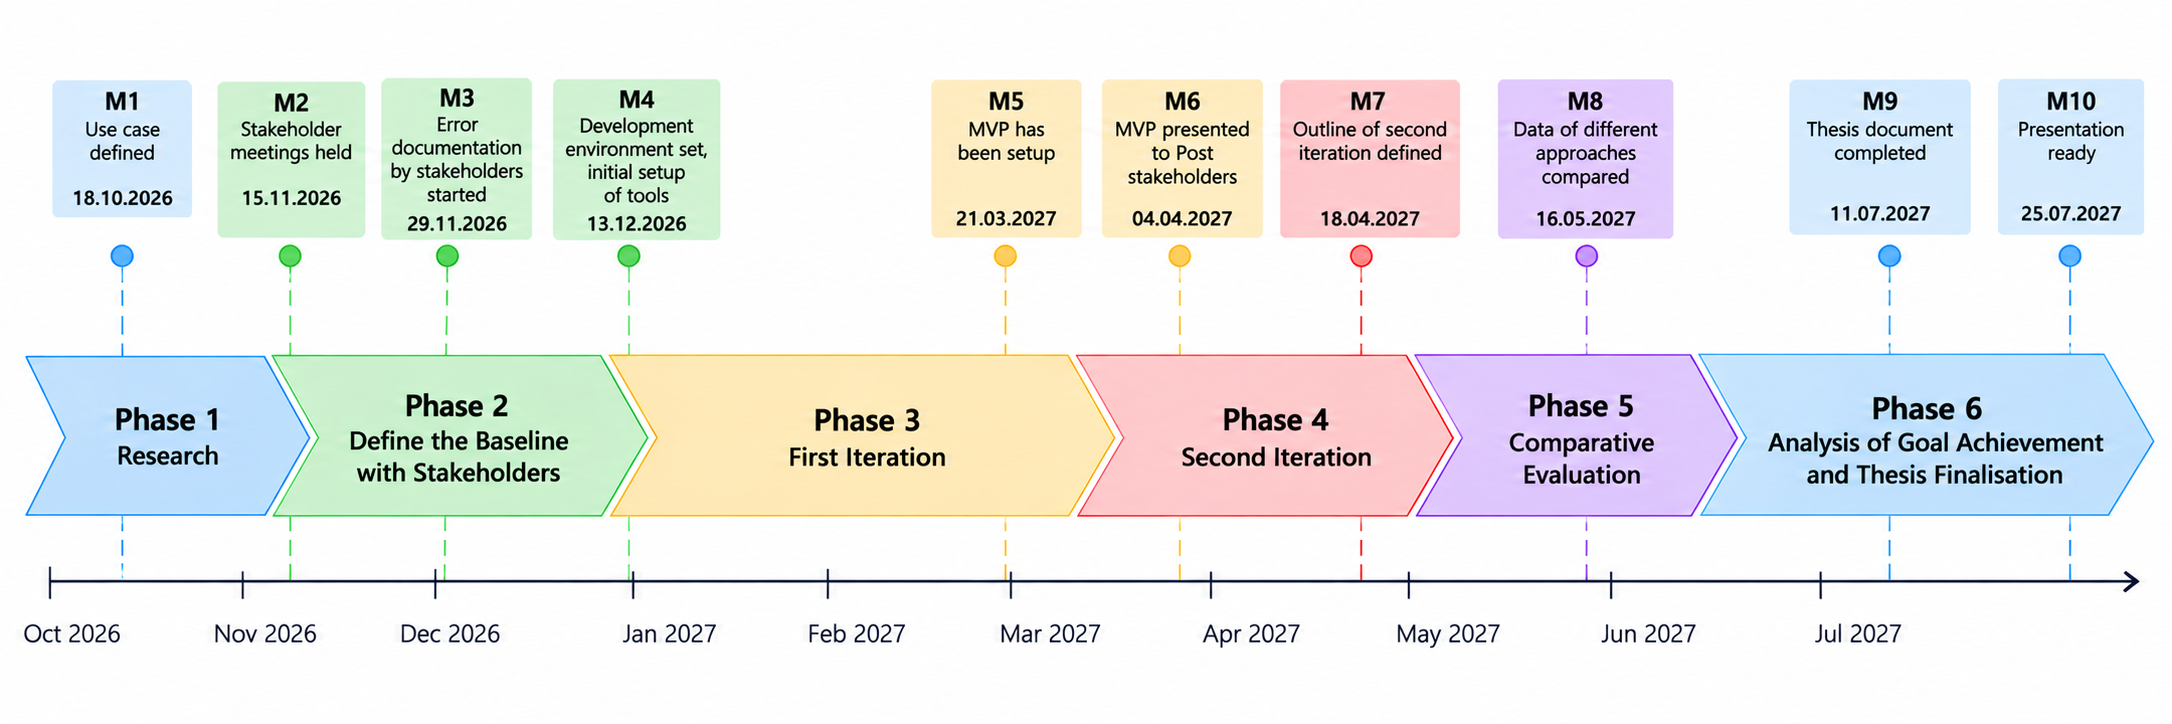
\includegraphics[width=0.8\textwidth]{./content/img/Mth/ProjectManagement/MilestoneTimelineAdapted_2.png}
    \caption{Milestones and phases defined at the start of the project}
    \label{fig:projmgmt_milestones_and_phases}
\end{figure}

